\section{Justificación}

% \defaultFontEpigraph{All You Need Is Beyond a Good Init}{\cite{xieAllYouNeed2017}}

% \defaultFontEpigraph{All You Need Is Beyond a Good Init}{Xie, Xiong, y Pu (2017)}

La evolución de la \gls{ia}, específicamente en el dominio del Aprendizaje Profundo o \gls{dl}, ha llevado al desarrollo de <<Modelos de Lenguaje a Gran Escala>> o \gls{llm}. Estos modelos, originalmente diseñados para emular el lenguaje humano, y conocidos por el gran público a través de aplicaciones tipo \emph{chatbot}\footnote{Entre las aplicaciones de \emph{chatbot} más conocidas están ChatGPT, Claude, Bart o Copilot, aunque la lista cada vez es más larga e incluye modelos de lenguaje de código abierto como LLaMa, Mistral o Falcon, entre otros.} han demostrado capacidades emergentes en áreas relacionadas con la creatividad y el razonamiento. Su éxito se extiende a sectores diversos como la literatura, el arte visual, la investigación, el marketing y la educación, afectando prácticamente a todas las disciplinas que involucran el uso del lenguaje o el razonamiento.

Contrario a las expectativas iniciales, los \gls{llm} han probado ser especialmente eficaces en la generación de código de programación, lugar donde podemos incluir lenguajes relacionados con la creación musical o sonora, siempre que el modelo haya contado para su entrenamiento con suficiente material escrito en el lenguaje en cuestión.

% No obstante, la generación de música mediante representaciones simbólicas (no sonoras en sí mismas) plantea retos significativos para los \gls{llm}. Tal generación musical requiere un conocimiento profundo de teoría musical, armonía y contrapunto, además de la capacidad de razonar sobre estos conceptos, lo cual actualmente no es una premisa en los \gls{llm} de uso general, no especializados en música.

Hay de señalar que existe una vertiente de desarrollo de modelos para la generación de audio, como \emph{Stability Audio}, \emph{MusicML} de Google y \emph{AWS DeepComposer} de Amazon. Dichos modelos generan música (audio) a partir de texto natural, mostrando resultados muy prometedores ---particularmente para el marketing y la creación de contenido--- por la potencial reducción de costos de producción. Sin embargo, los archivos de audio generados son inalterables y escapan al control humano, lo cual limita su aplicación en composición musical donde, entendemos, la intervención humana es esencial\footnote{No se entrará en el debate de si puede considerarse o no como arte un producto de un modelo de \gls{ia}. En nuestro estudio se partirá del postulado de que el factor creador humano es quien decide que un producto sea o no arte.}. En contraste, los \gls{llm} generan texto, incluso texto musical, lo que permite la edición y el control por parte del compositor, y abre, así, amplias posibilidades de interacción humano-máquina en el proceso creativo.

Se han realizado estudios sobre la capacidad de los \gls{llm} para generar algoritmos en lenguajes de programación enfocados en la resolución de problemas matemáticos y el desarrollo de \emph{software}, campo en el que los \gls{llm} han mostrado una elevada efectividad. No obstante, existe una carencia en lo que respecta al estudio de la generación de código musical con finalidad artística, alineado con las intenciones del creador sonoro o compositor. No es equiparable desarrollar, por ejemplo, un código que muestre el conjunto de Mandelbrot (véase Figura \ref{fig:python_mandelbrot}) con crear un código inspirado en dicho fractal (véase Figura \ref{fig:supercollider_mandelbrot}). Al contrario de lo que se podría intuir en un primer momento, el segundo caso requiere, con creces, de un nivel superior de comprensión, abstracción, conocimientos previos y conexión con la realidad que el primero, incluso si su código puede ser eventualmente más simple que el de la función matemática. Por ello, resulta fundamental realizar estudios específicos que exploren la capacidad de los \gls{llm} en la generación de código musical con finalidad artística.

\begin{figure}%[H]
    \caption[Generación de código matemático en Python con ChatGPT (GPT-4)]{Generación de código matemático en Python con ChatGPT (GPT-4). La petición es simple, pero el procedimiento a seguir es complejo. El resultado se muestra en la imagen inferior, que resultó completamente exitosa en un solo intento.}
      \centering
      \begin{mdframed}
        \setstretch{1}
        \fontsize{9.5pt}{11pt}\selectfont
        Usuario: Crea un código en Python que dibuje el conjunto de Mandelbrot.
      \end{mdframed}
        \centering
        \setstretch{1}
        \begin{mdframed}
          \setstretch{1}
          \fontsize{9.5pt}{11pt}\selectfont
        \begin{lstlisting}[language=Python, basicstyle=\footnotesize\ttfamily, keywordstyle=\color{blue}, commentstyle=\color{green}, stringstyle=\color{red},
        numbers=none]
import numpy as np
import matplotlib.pyplot as plt

def mandelbrot(c, max_iter):
    z = 0
    for n in range(max_iter):
        if abs(z) > 2:
            return n
        z = z*z + c
    return max_iter

# Crear una imagen del conjunto de Mandelbrot
columns = 800
rows = 600
result = np.zeros((rows, columns))

# Rango de valores para x e y
x_min, x_max = -2.0, 1.0
y_min, y_max = -1.5, 1.5

# Máximo número de iteraciones
max_iter = 256

# Generar valores para cada punto de la imagen
for row_index, Re in enumerate(np.linspace(y_min, y_max, num=rows)):
    for column_index, Im in enumerate(np.linspace(x_min, x_max, num=columns)):
        c = complex(Im, Re)
        result[row_index, column_index] = mandelbrot(c, max_iter)

# Mostrar la imagen
plt.figure(figsize=(8, 6))
plt.imshow(result, cmap='hot', extent=[x_min, x_max, y_min, y_max])
plt.colorbar()
plt.title('Conjunto de Mandelbrot')
plt.xlabel('Re')
plt.ylabel('Im')
plt.show()              
        \end{lstlisting}
      \end{mdframed}
        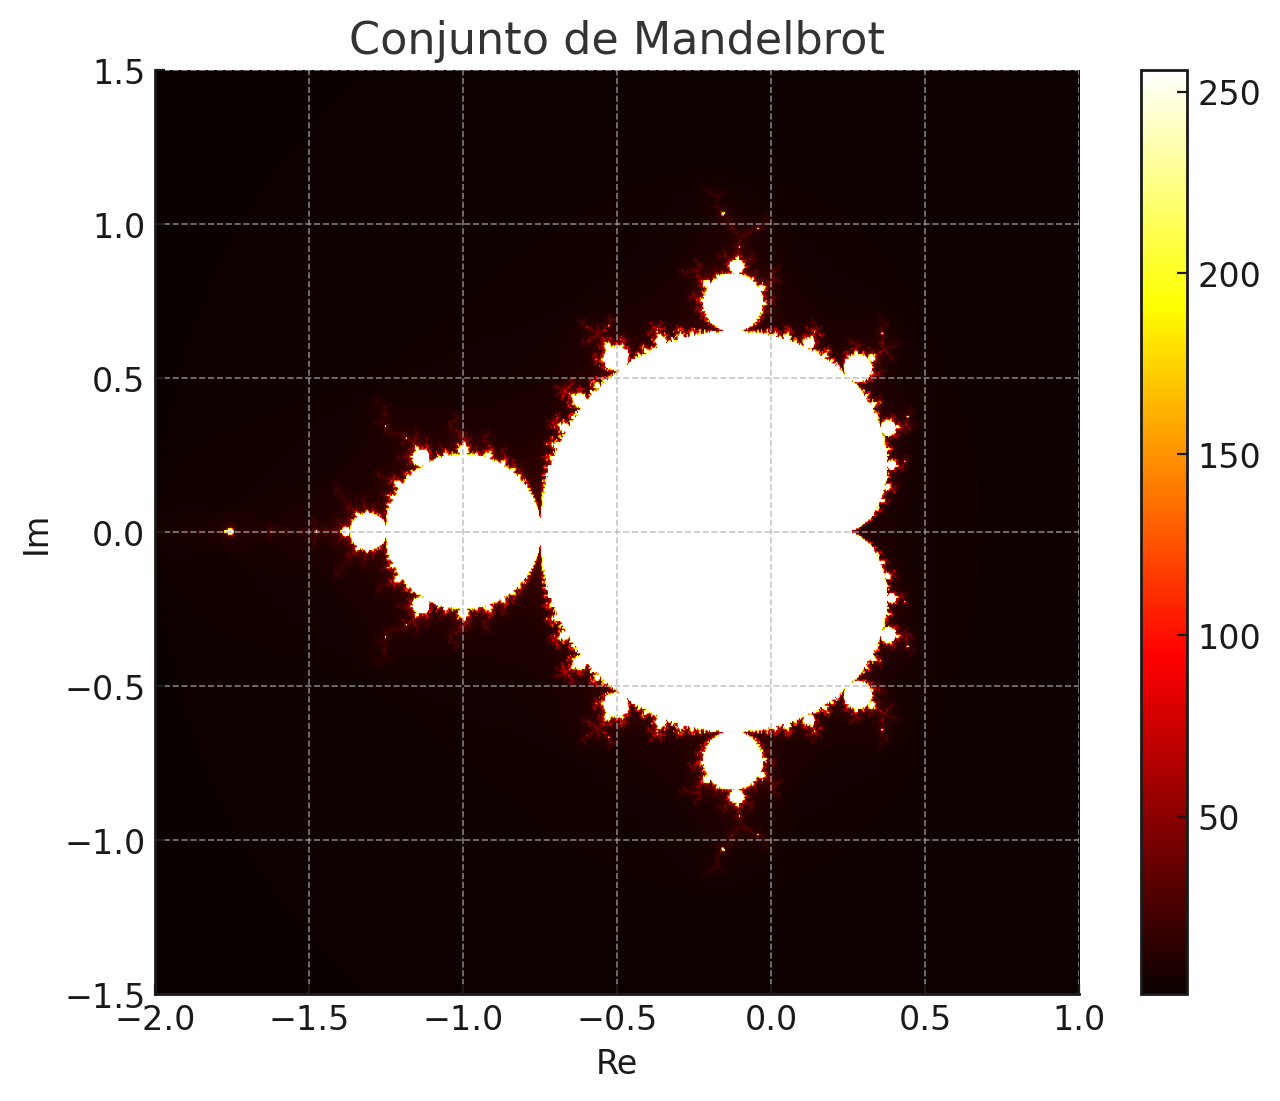
\includegraphics[width=0.7\textwidth]{./figuras/python_mandelbrot.png}
    \source{\propio}
    \label{fig:python_mandelbrot}
\end{figure}


\begin{figure}%[H]
  \caption[Código en SuperCollider generado por ChatGPT (GPT-4)]{Código en SuperCollider generado por ChatGPT (GPT-4). Al contrario que en la Figura \ref{fig:python_mandelbrot}, la complejidad no reside en el código en sí sino en la abstracción de lo que se pide y la dificultad de generar un producto artístico.}
  \vspace{-.5cm}
  \captionqranexo{\hspace{9cm}}{https://drive.google.com/file/d/1l2VpDqor6xFkxHc5jnxqQiszuUieIPVw/view?usp=sharing}{audio}
  \vspace{.2cm}
  \centering
    \begin{mdframed}
      \setstretch{1}
      \fontsize{9.5pt}{11pt}\selectfont
      Usuario: Crea una textura sonora de interés artístico usando \texttt{FMGrain} en SuperCollider.
    \end{mdframed}
    \centering
      \setstretch{1}
      \begin{lstlisting}[style=SuperCollider-IDE, basicstyle=\footnotesize\ttfamily, numbers=none]
(
  SynthDef(\mandelbrotSound, {
      arg out=0, freq=440, dur=2, amp=0.1;
      var env, signal, modFreq;
  
      // Envolvente para controlar la amplitud general del sonido
      env = EnvGen.kr(Env.perc(0.01, dur, amp, -4), doneAction:2);
  
      // Frecuencia de modulación basada en una relación matemática
      modFreq = SinOsc.kr(0.2, 0, 20, freq);
  
      // Genera una textura sonora con múltiples osciladores
      signal = Mix.fill(8, {
          arg i;
          var freqMod;
          freqMod = modFreq * (i+1) * Rand(0.9!2, 1.1);
          SinOsc.ar(freqMod, 0, env * (1/(i+1)))
      });
  
      Out.ar(out, signal);
  }).add;
  
  // Tocar el sonido con diferentes frecuencias base
  Pbind(
      \instrument, \mandelbrotSound,
      \freq, Pseq([220, 330, 440, 550], inf),
      \dur, 0.5
  ).play;
)       
      \end{lstlisting}
  
  \source{\propio}
  \label{fig:supercollider_mandelbrot}
\end{figure}


Un aspecto muy importante a investigar a la hora de estudiar la utilidad e influencia de sistemas de \gls{ia} en la creación artística es el de la \emph{interfaz} entre el este y el artista. La interfaz es el medio por el cual el artista interactúa con el sistema, y puede ser de muy diversa índole. En el caso de los \gls{llm}, la interfaz más común es la \emph{chatbot}, donde el artista se comunica en forma de diálogo en lenguaje natural. Sin embargo, existen otras interfaces que pueden ser más adecuadas para la creación musical, como la interfaz gráfica, la interfaz de voz o la interfaz gestual, etc.

Aunque existen numerosos lenguajes de programación enfocados en la creación musical relevantes para este estudio, la investigación se centrará en dos de ellos por limitaciones de espacio. El principal será \emph{SuperCollider}, un lenguaje consolidado para síntesis sonora y procesamiento de audio, que ofrece un entorno propicio para esta investigación por su riqueza expresiva y reconocimiento en la comunidad de música electrónica y experimental. El segundo, \emph{Tidal Cycles}, se basa en la filosofía de la improvisación sonora en interpretaciones en vivo o \emph{Live Coding}, lo cual permite la exploración de interfaces innovadoras. La combinación de las capacidades de codificación de los \gls{llm} con la versatilidad de estos lenguajes promete un panorama lleno de posibilidades creativas. Este estudio pretende investigar dicho panorama, buscando comprender cómo la creatividad emergente de los \gls{llm} se manifiesta en la composición musical algorítmica y cómo esta interacción puede ampliar las fronteras de la música digital. Los resultados serán aplicables a cualquier lenguaje estructurado orientado a la creación sonora o musical, como \emph{Overtone}, \emph{Pure Data} y \emph{Sonic Pi}, entre otros.

Este trabajo busca aportar al mundo de la música, en concreto del arte sonoro, una nueva perspectiva sobre la creación musical, apoyada en la investigación en \gls{ia}, para expandir las fronteras de la creatividad y explorar interfaces innovadoras entre el artista y la máquina. Aspiramos a que sea una invitación a la experimentación y la investigación en este campo en rápido desarrollo.

Asimismo, se espera que la comunidad científica de la \gls{ia} encuentre en este estudio una retroalimentación valiosa desde la investigación musical, contribuyendo a mejorar los modelos de \gls{ia} y sus aplicaciones prácticas. Adicionalmente, este trabajo busca incentivar la investigación y desarrollo de \gls{llm} \emph{open source}, lo cual fomentará la colaboración futura entre las comunidades científica y artística en la creación de tecnologías abiertas para la creación musical y sonora.